\documentclass[11pt,a4paper]{article}
\usepackage[margin=2.3cm]{geometry}
\usepackage[T1]{fontenc}
\usepackage{amsmath,amssymb}
\usepackage{booktabs,tabularx,array}
\usepackage{enumitem}
\usepackage{xcolor}
\usepackage{listings}
\usepackage{tikz}
\usetikzlibrary{positioning,arrows.meta,shapes.geometric}
\usepackage[colorlinks=true,linkcolor=blue!50!black,urlcolor=blue!50!black]{hyperref}

\setlist{itemsep=2pt,topsep=3pt}
\newcolumntype{Y}{>{\raggedright\arraybackslash}X}
\lstset{basicstyle=\ttfamily\footnotesize,breaklines=true,frame=single,backgroundcolor=\color{black!3},columns=fullflexible}
\newcommand{\code}[1]{\texttt{#1}}
\newcommand{\todo}[1]{\textcolor{red!60!black}{[#1]}}

\title{\textbf{Training Pipeline, Resources and Deliverables}\\[2pt]
\large Counterfactual Relational Video Anomaly Detection through\\ Minimal-Intervention Contrastive Learning}
\author{Planning document for the capstone (Ashwin V, Madhu Shraya)\\
Compute budget: 2$\times$ NVIDIA A40 (48\,GB each)}
\date{Draft, 10 October 2026}

\begin{document}
\maketitle

\begin{abstract}
\noindent This document turns the Phase~1 idea (matched factual/counterfactual event pairs, one factor changed at a time) into a concrete training pipeline for two A40 GPUs: what to train, in which order, on which data, what it costs, what to deliver, and when to stop. The design keeps all large encoders \emph{frozen} and trains only small heads on precomputed features, so the real cost is data (pseudo-labelling and a small controlled evaluation set), not GPU time. A code skeleton accompanies this document. \textbf{Verification status:} the code was exercised end-to-end only on synthetic features; GPU-side feature extraction and the VLM backend are written but untested, dataset sizes are quoted from memory, and every compute figure is a planning estimate to be replaced by measurements from the pilot (Appendix~\ref{sec:status}).
\end{abstract}

%------------------------------------------------------------------
\section{Scope and design decisions}
The research question is whether a weakly supervised VAD model can learn \emph{which factor change} makes an event abnormal. Three decisions from the earlier discussion shape everything below.

\begin{enumerate}
\item \textbf{Closed slot schema.} An event is a tuple (action, object, scene, relation). With $8\times6\times6\times6=1728$ values the whole hypothesis space is enumerable, every hypothesis sentence can be embedded once (a \emph{text bank}), and a ``minimal intervention'' is exact: one slot index differs. The schema in the code is a placeholder; finalize it after the pilot (Stage~0).
\item \textbf{Compatibility is not anomaly.} A video--hypothesis match score alone says nothing about abnormality. The model therefore has two parts: a \emph{grounding} part (video $\leftrightarrow$ hypothesis similarity) and a \emph{normality head} that judges the described slot tuple. The anomaly score of a segment is the expected abnormality under the segment's hypothesis posterior (Section~\ref{sec:model}).
\item \textbf{Frozen encoders, small heads.} Video features come from a frozen CLIP image encoder and hypotheses from the CLIP text encoder; only a temporal adapter, a text projection and the normality head train (about 2.3 million parameters at the default width). The Qwen-class VLM is used \emph{only} to produce pseudo-labels, not at inference.
\end{enumerate}

%------------------------------------------------------------------
\section{Requirements}
\subsection{Hardware and software}
\begin{tabularx}{\linewidth}{@{}l Y@{}}
\toprule
Item & Requirement / note\\
\midrule
GPUs & 2$\times$ A40, 48\,GB each (Ampere, supports bf16). No NVLink assumed; the pipeline never needs multi-GPU gradient synchronization: GPU~0 and GPU~1 run \emph{independent shards or independent runs}.\\
CPU / RAM & Video decoding is the likely bottleneck in feature extraction. Plan for as many CPU cores as you can get and $\ge$64\,GB RAM; measure on the pilot.\\
Disk & Reserve $\ge$1\,TB for raw videos and caches (planning figure; check the actual download sizes). Derived features are small (Section~\ref{sec:compute}).\\
Software & Python 3.10+, PyTorch $\ge$2.2, \code{transformers}, \code{qwen-vl-utils}, OpenCV, scikit-learn, PyYAML (see \code{requirements.txt}). A vLLM server is optional for faster pseudo-labelling.\\
Frozen models & CLIP ViT-B/16 (image+text); a 7B-class VLM (e.g.\ Qwen2-VL-7B-Instruct) for Stage~0 only.\\
\bottomrule
\end{tabularx}

\subsection{Data and external resources}
\label{sec:data}
Sizes below are approximate and from memory; \textbf{verify sizes and licences before downloading} (several of these are research/non-commercial and some require a request form).

\begin{tabularx}{\linewidth}{@{}l Y Y@{}}
\toprule
Resource & Role in the pipeline & Notes\\
\midrule
UCF-Crime & Weak-label VAD training (Stage~2) and final testing & $\approx$1.9k untrimmed videos, 13 classes, $\approx$128\,h. Low resolution.\\
XD-Violence & Stage~2 training / testing & $\approx$4.8k videos, $\approx$217\,h; audio available (unused).\\
ShanghaiTech Campus & Testing; scene-level normality & Small, fixed cameras; anomalies are mostly ``non-pedestrian'' or fast motion.\\
UBnormal & Synthetic scenes; candidate base for controlled pairs & Unity-rendered, pixel-level labels; domain gap to real video.\\
MSAD (optional) & Extra scene diversity & Check availability and licence.\\
Something-Something V2 & Stage~1 relational pretraining: \emph{real} minimal pairs (put into / take out of, covering / uncovering) & $\approx$220k clips, 174 template classes. Map templates to (action, object, relation) slots.\\
Something-Else (annotations) & Compositional splits (unseen action--object combinations) & Annotations over SSv2; use for the held-out-composition protocol.\\
UCA / CUVA / HIVAU & Language seeds for factor wording; sanity check of pseudo-labels & Free-form text, so mapping to slots is still needed.\\
Controlled pair set (\emph{build it}) & Evaluation only: matched video pairs differing in one factor & Target 300--500 pairs, two annotators, inter-annotator agreement reported. Sources: staged recordings, simulator, or mined near-duplicates.\\
Human audit sample (\emph{build it}) & Measure pseudo-label noise & 300--500 clips labelled by hand on the slot schema.\\
\bottomrule
\end{tabularx}

%------------------------------------------------------------------
\section{Training pipeline}
\label{sec:pipeline}

\begin{figure}[h]
\centering
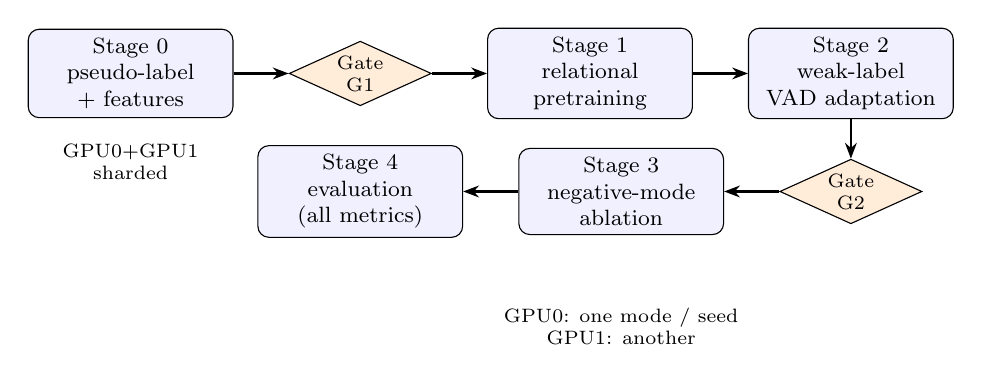
\begin{tikzpicture}[
  node distance=5mm and 7mm,
  box/.style={draw,rounded corners,align=center,minimum width=2.6cm,minimum height=1.0cm,font=\footnotesize,fill=blue!6},
  gate/.style={draw,diamond,aspect=2.2,align=center,font=\scriptsize,fill=orange!15,inner sep=1pt},
  arr/.style={-{Stealth[length=2mm]},thick}]
\node[box] (s0) {Stage 0\\pseudo-label\\+ features};
\node[gate,right=of s0] (g1) {Gate\\G1};
\node[box,right=of g1] (s1) {Stage 1\\relational\\pretraining};
\node[box,right=of s1] (s2) {Stage 2\\weak-label\\VAD adaptation};
\node[gate,below=of s2] (g2) {Gate\\G2};
\node[box,left=of g2] (s3) {Stage 3\\negative-mode\\ablation};
\node[box,left=of s3] (s4) {Stage 4\\evaluation\\(all metrics)};
\draw[arr] (s0) -- (g1); \draw[arr] (g1) -- (s1); \draw[arr] (s1) -- (s2);
\draw[arr] (s2) -- (g2); \draw[arr] (g2) -- (s3); \draw[arr] (s3) -- (s4);
\node[font=\scriptsize,align=center,below=2mm of s0] {GPU0+GPU1\\sharded};
\node[font=\scriptsize,align=center,below=2mm of s3,yshift=-6mm] {GPU0: one mode / seed\\GPU1: another};
\end{tikzpicture}
\caption{Pipeline with two decision gates. Stage~0 shards across both GPUs; Stages~1--3 run independent jobs on each GPU.}
\end{figure}

\subsection*{Stage 0 -- Factor pseudo-labelling and feature extraction (both GPUs, sharded)}
\begin{enumerate}
\item \textbf{Windows.} Cut each surveillance video into windows of $T{=}32$ segments, each segment the mean CLIP feature of 8 frames sampled at 2\,fps (4\,s per segment, $\approx$128\,s per window). For SSv2 use short clips with $T{=}8$.
\item \textbf{Nuisance view.} For every window also encode one augmented view (random-resized crop, colour jitter; one random draw per window). These pairs drive the invariance loss and the stability metric. Stronger, scene-level nuisances (background swap) need pixel-space edits and are optional.
\item \textbf{Pseudo-labels.} Prompt the VLM to fill the closed schema (JSON only), sample $N{=}3$ answers per window, take a per-slot majority, and define confidence as the mean per-slot agreement. Windows with an unresolved slot get no hypothesis.
\item \textbf{Human audit (gate G1).} Hand-label 300--500 windows. Report per-slot agreement overall and by confidence bucket. Drop or merge slots whose agreement is poor; use only confident labels in Stage~2.
\item \textbf{Text bank.} Embed all 1728 hypothesis sentences with the CLIP text encoder once.
\end{enumerate}

\subsection*{Stage 1 -- Relational pretraining (one A40, minutes--hours)}
Train adapter, text projection and logit scale with a candidate InfoNCE loss on clips whose slot tuple is known (SSv2 mapped to slots). Negatives are drawn per the chosen mode (Section~\ref{sec:model}). Add the margin and invariance terms. Hold out (action, object) combinations for the compositional metric. The normality head is \emph{not} trained here, since SSv2 has no notion of abnormal.

\subsection*{Stage 2 -- Weak-label VAD adaptation (one A40)}
Initialize from Stage~1. Train on weakly labelled surveillance windows with: (i) MIL loss on the anomaly score from the video-level label, so the normality head learns \emph{only} from weak labels; (ii) confidence-weighted InfoNCE on the pseudo-hypothesis with the same negative mode; (iii) invariance. The weak ABNORMAL\_RULES prior is off by default (\code{lam\_rule=0}) to avoid injecting a hand-written definition of abnormality into the main results.

\subsection*{Stage 3 -- The decisive ablation (gate G2)}
Run the same pipeline with the three negative modes (random / multi-slot / single-slot), $\ge$3 seeds each, matched data volume and steps. This is the experiment that justifies the thesis, so run it \emph{early} on a subset; see gates in Section~\ref{sec:deliver}.

\subsection*{Stage 4 -- Evaluation}
Standard metrics on the benchmarks plus intervention, nuisance and compositional metrics on the controlled pair set (Section~\ref{sec:eval}). Checkpoints are chosen on a validation split of the \emph{training} source only.

%------------------------------------------------------------------
\section{Model and objectives}
\label{sec:model}
Let $x\in\mathbb{R}^{T\times D}$ be segment features, $g_\theta$ the temporal adapter producing unit-norm segment embeddings $v_t$, and $u_h$ the unit-norm projected text embedding of hypothesis $h$ in the bank $\mathcal H$ ($|\mathcal H|{=}1728$).

\paragraph{Grounding.} Clip--hypothesis similarity is $s(x,h)=\max_t \langle v_t,u_h\rangle$, because the event may occupy only part of a window.

\paragraph{Normality and anomaly score.} A head over concatenated slot embeddings gives $a(h)=\sigma(f_\phi([e_1(h_1),\dots,e_4(h_4)]))$. The segment score is the posterior expectation
\begin{equation}
 p(h\mid t)=\operatorname{softmax}_{h}\big(\lambda\langle v_t,u_h\rangle\big),\qquad
 \text{score}_t=\sum_{h\in\mathcal H}p(h\mid t)\,a(h),
\end{equation}
and the video score is the mean of the top-$k$ segment scores ($k=T/8$).

\paragraph{Losses.} For an anchor with positive hypothesis $h^+$ and $K$ sampled negatives $\mathcal N$,
\begin{align}
\mathcal L_{\text{nce}} &= -\log\frac{e^{\lambda s(x,h^+)}}{e^{\lambda s(x,h^+)}+\sum_{h^-\in\mathcal N}e^{\lambda s(x,h^-)}},\\
\mathcal L_{\text{margin}} &= \big[m-\big(s(x,h^+)-\max_{h^-\in\mathcal N}s(x,h^-)\big)\big]_+,\\
\mathcal L_{\text{inv}} &= 1-\tfrac1T\textstyle\sum_t\langle v_t(x),v_t(\tilde x)\rangle,\\
\mathcal L_{\text{MIL}} &= \operatorname{BCE}\big(\text{top-}k\text{ mean}_t\,\text{score}_t,\; y_{\text{video}}\big).
\end{align}
Stage 1 minimizes $\mathcal L_{\text{nce}}+0.5\,\mathcal L_{\text{margin}}+0.5\,\mathcal L_{\text{inv}}$. Stage 2 minimizes $\mathcal L_{\text{MIL}}+0.5\,\mathcal L_{\text{nce}}+0.25\,\mathcal L_{\text{margin}}+0.5\,\mathcal L_{\text{inv}}$ (weights are starting points, to be tuned on the validation split).

\paragraph{Negative modes (the manipulated variable).}
\textbf{random:} uniformly random hypotheses (the LAVIDA-style decoy). \textbf{multi:} 2--4 slots changed at once (an approximation of curated semantic hard negatives; read the Alert-CLIP construction before claiming equivalence). \textbf{single:} exactly one slot changed (minimal intervention).

\paragraph{Known limitation.} Training uses $K{=}16$ sampled candidates but inference takes the softmax over all 1728 hypotheses; the posterior may therefore be miscalibrated. If it is, restrict the posterior to a top-$M$ candidate set or train with larger $K$.

%------------------------------------------------------------------
\section{Compute, storage and time budget}
\label{sec:compute}
All times are \textbf{unmeasured planning estimates}; replace them with pilot measurements.

\begin{tabularx}{\linewidth}{@{}l Y Y@{}}
\toprule
Item & Estimate & Reasoning\\
\midrule
Feature windows & 32\,KiB per window per view & $32\times512\times2$\,B in fp16; 100k windows $\times$ 2 views $\approx$ 6.5\,GB.\\
SSv2 features & $\approx$3.6\,GB for two views & $\approx$220k clips $\times$ $8\times512\times2$\,B $\approx$ 1.8\,GB per view.\\
Frames to encode & $\approx$4--5\,M & $\approx$350\,h surveillance at 2\,fps $\approx$2.5\,M, plus $\approx$1.8\,M for SSv2.\\
Feature extraction & GPU $\approx$1--2\,h; wall-clock $\approx$1 day & GPU time is small; decoding on the CPU dominates. Shard 0/2 and 1/2.\\
VLM memory & $\approx$17\,GB weights per replica & Fits one A40 per replica with headroom; run one replica per GPU.\\
Pseudo-labelling & $\approx$14\,h wall for 20k windows $\times$ 3 samples & Assumes $\sim$5\,s per window per GPU; \emph{measure on 50 windows first}; vLLM can cut this a lot.\\
Stage 1 / Stage 2 head training & well under 1 GPU-hour per run & Tiny heads on cached features; $<$2\,GB GPU memory expected.\\
Ablation grid & $\approx$18 runs ($3$ modes $\times$ 3 seeds $\times$ 2 stages) $\approx$ $\le$18 GPU-h & $\approx$9\,h wall with one independent run per GPU.\\
\bottomrule
\end{tabularx}
\label{tab:compute}

\medskip\noindent\textbf{Why not train the encoders?} Fine-tuning the CLIP encoders (e.g.\ with LoRA) would fit on 2 A40s, but it multiplies cost and confounds the negative-mode ablation. Treat it as an optional extension only after gate G2.

%------------------------------------------------------------------
\section{Experimental protocol}
\label{sec:eval}
\subsection{Metrics}
\begin{tabularx}{\linewidth}{@{}l Y@{}}
\toprule
Metric & Definition\\
\midrule
Video AUC / AP & Detection from the top-$k$ segment score on UCF-Crime, XD-Violence, ShanghaiTech (use the benchmark's standard protocol for frame-level numbers).\\
Edit accuracy (grounding) & $\Pr[s(x,h_{\text{true}})>s(x,h_{\text{edit}})]$ over all 22 single-slot edits, reported per slot.\\
Flip accuracy (intervention) & On matched pairs, $\Pr[\text{score(abnormal)}>\text{score(normal)}]$.\\
Nuisance stability & $\mathbb{E}|\text{score}(x)-\text{score}(\tilde x)|$ and flip accuracy on nuisance views.\\
Compositional generalization & All of the above on held-out (action, object) combinations vs.\ seen ones.\\
\bottomrule
\end{tabularx}

\subsection{Baselines and ablations}
\begin{tabularx}{\linewidth}{@{}l Y@{}}
\toprule
Run & Purpose\\
\midrule
Text-only (no video) and shuffled-video & Detect hypothesis-only bias; if either beats chance on the pair set, the benchmark is broken.\\
Zero-shot CLIP similarity & Floor for grounding without training.\\
random / multi / single negatives & The central claim; matched data volume, $\ge$3 seeds, report mean and spread.\\
No invariance loss & Isolates the nuisance-stability contribution.\\
No normality head (compatibility only) & Shows why compatibility is not anomaly.\\
Published VAD baselines & Only compare numbers under the same protocol; do not copy table values across protocols.\\
\bottomrule
\end{tabularx}

\subsection{Protocol rules}
\begin{itemize}
\item Never select checkpoints or tune hyperparameters on a test benchmark; use a validation split of the training source.
\item Freeze the slot schema and normality conventions \emph{before} building the controlled pair set; have annotators verify each pair.
\item Report the pseudo-label noise estimate next to every result that depends on it.
\end{itemize}

%------------------------------------------------------------------
\section{Deliverables and decision gates}
\label{sec:deliver}
\begin{tabularx}{\linewidth}{@{}l Y Y@{}}
\toprule
Milestone & Deliverables & Acceptance / gate (suggested thresholds)\\
\midrule
M0 Pilot (Stage 0 on $\sim$50--200 clips) & Final slot schema; labelled audit sample (300 clips); pseudo-label agreement report & \textbf{G1:} per-slot human agreement high enough to use (suggest $\ge$0.7 on slots kept); drop slots below it.\\
M1 Data & Feature caches (surveillance + SSv2, two views); text bank; \code{stage1/2\_train.pt}; controlled pair set with agreement stats & Pair set passes text-only and shuffled-video checks (near chance).\\
M2 Stage 1 & Trained relational checkpoint; edit accuracy per slot on seen and held-out combos & Held-out edit accuracy clearly above zero-shot CLIP.\\
M3 Stage 2 + ablation & Checkpoints for 3 modes $\times$ 3 seeds; ablation table & \textbf{G2:} single-slot beats random \emph{and} multi-slot on flip / held-out metrics beyond seed spread. If not, the gap claim fails; pivot (e.g.\ a compositional-grounding study) instead of polishing.\\
M4 Final & Full results on all benchmarks and controlled set; failure analysis; code release with README; capstone report & Reproducible from configs; results table regenerated by one script.\\
\bottomrule
\end{tabularx}

%------------------------------------------------------------------
\section{Risks and open issues}
\begin{itemize}
\item \textbf{Pseudo-label noise} can dominate; any gain may partly be agreement with the labelling VLM. Mitigate with confidence weighting, human audit, and a second VLM as a cross-check.
\item \textbf{Weakly visible factors} (ownership, authorization) often cannot be recovered from pixels; prefer visually grounded relations (source location, direction, contact, sequence).
\item \textbf{Benchmarks may not show gains.} UCF-Crime and XD-Violence are dominated by coarse anomalies; the intervention and compositional metrics must carry the contribution.
\item \textbf{Domain gap} between SSv2 (egocentric, close-up) and surveillance may weaken Stage~1 transfer; test on a small subset early.
\item \textbf{Prior-art claims} about Fine-VAD and Alert-CLIP negative construction are unverified here; read those sections before writing the gap argument.
\item \textbf{Schema ceiling.} A closed schema limits the anomalies expressible; state this as a scope limitation.
\end{itemize}

%------------------------------------------------------------------
\section{Indicative schedule}
The capstone calendar is unknown, so this assumes 14 weeks; shift as needed.
\begin{center}
\begin{tabularx}{\linewidth}{@{}l Y@{}}
\toprule
Weeks & Work\\
\midrule
1--2 & Environment, dataset access, schema draft, Stage~0 pilot and audit (G1).\\
3--5 & Bulk feature extraction and pseudo-labelling; build controlled pair set; text/shuffled baselines.\\
6--7 & Stage~1 pretraining; Stage~2 on a subset; \textbf{early ablation (G2)}.\\
8--10 & Full ablation grid, seeds, remaining ablations.\\
11--12 & Benchmarks, failure analysis, optional extension.\\
13--14 & Write-up, code cleanup, reproducibility check.\\
\bottomrule
\end{tabularx}
\end{center}

%------------------------------------------------------------------
\appendix
\section{Repository layout and commands}
\begin{lstlisting}
crvad/slots.py         slot schema, single-slot edits, compositional split
crvad/model.py         temporal adapter, text projection, normality head
crvad/losses.py        negative samplers, InfoNCE+margin, invariance, MIL
crvad/train.py         stage 1 and stage 2 training
crvad/evaluate.py      AUC/AP, edit/flip/nuisance/held-out metrics
crvad/pseudo_label.py  VLM slot labelling, voting, audit export
crvad/features.py      CLIP features (+nuisance view), text bank
tests/smoke_test.py    synthetic end-to-end test
\end{lstlisting}
\begin{lstlisting}
python -m crvad.features text --out data/text_bank.pt
CUDA_VISIBLE_DEVICES=0 python -m crvad.pseudo_label --items items.jsonl --out l0.jsonl --shard 0/2
CUDA_VISIBLE_DEVICES=1 python -m crvad.pseudo_label --items items.jsonl --out l1.jsonl --shard 1/2
CUDA_VISIBLE_DEVICES=0 python -m crvad.train --stage 1 --set stage1.neg_mode=single out=runs/single_s0
CUDA_VISIBLE_DEVICES=1 python -m crvad.train --stage 1 --set stage1.neg_mode=random out=runs/random_s0
python -m crvad.evaluate --ckpt runs/single_s0/stage2/best.pt --text-bank data/text_bank.pt \
       --videos data/test_videos.pt --pairs data/pairs.pt
\end{lstlisting}

\section{Verification status}
\label{sec:status}
\begin{itemize}
\item \textbf{Run:} unit checks (slot encoding, one-slot edits, negative samplers), the pseudo-label parser/voting with a mock VLM, and an end-to-end Stage~1 $\rightarrow$ Stage~2 $\rightarrow$ evaluation on synthetic features (CPU).
\item \textbf{Synthetic result, read with care:} in the synthetic world (additive slot vectors) all three negative modes reached edit accuracy $\approx$1.0, video AUC $\approx$0.95 and flip accuracy $\approx$0.93--0.94. The test confirms the code path works; it \emph{cannot} separate the negative modes, so it says nothing about the thesis.
\item \textbf{Not run:} CLIP feature extraction, text-bank construction, the Qwen2-VL backend, any real dataset.
\item \textbf{From memory, to verify:} dataset sizes and licences; GPU throughput and all time estimates.
\end{itemize}

\end{document}
